\chapter{Конструкторская часть}

\section*{Схемы алгоритмов}

На рисунках 2.1 - 2.3 изображены схема алгоритма матричного алгоритма Левенштейна, схема рекурсивного алгоритма Дамерау-Левенштейна, схема рекурсивного алгоритма Дамерау-Левенштейна с кешированием соответственно.


\begin{figure}[ht!]
	\centering
	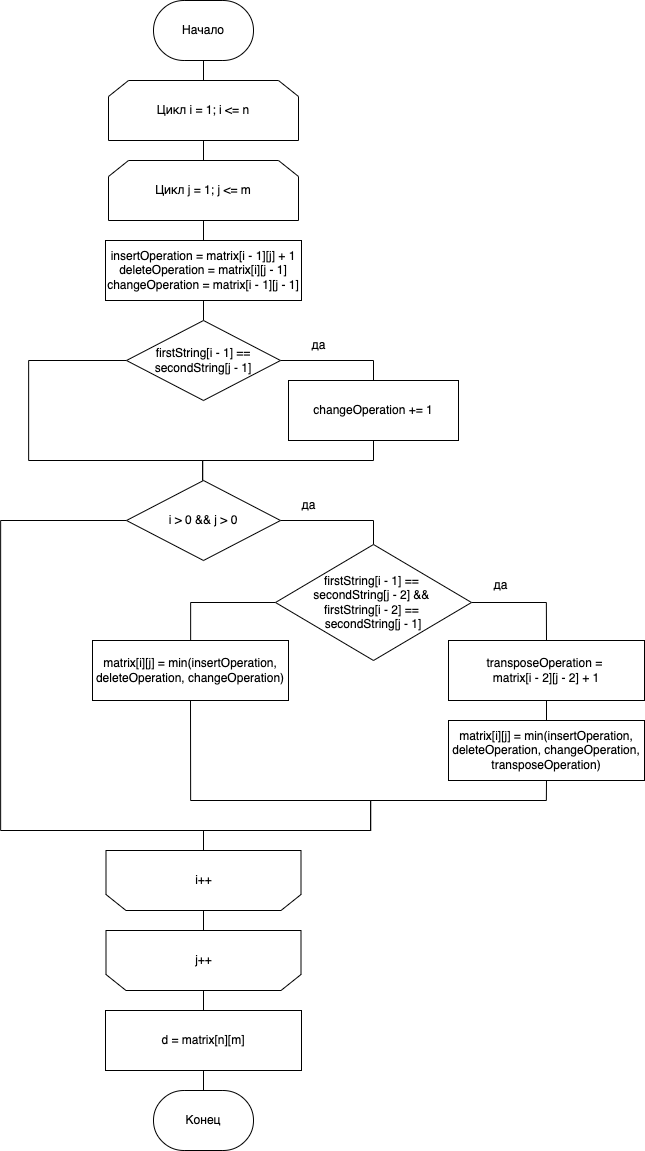
\includegraphics[width=0.83\linewidth]{img/dl_iter.png}
	\caption{Схема стандартного алгоритма умножения матриц}
	\label{fig:mpr}
\end{figure}

\begin{figure}[ht!]
	\centering
	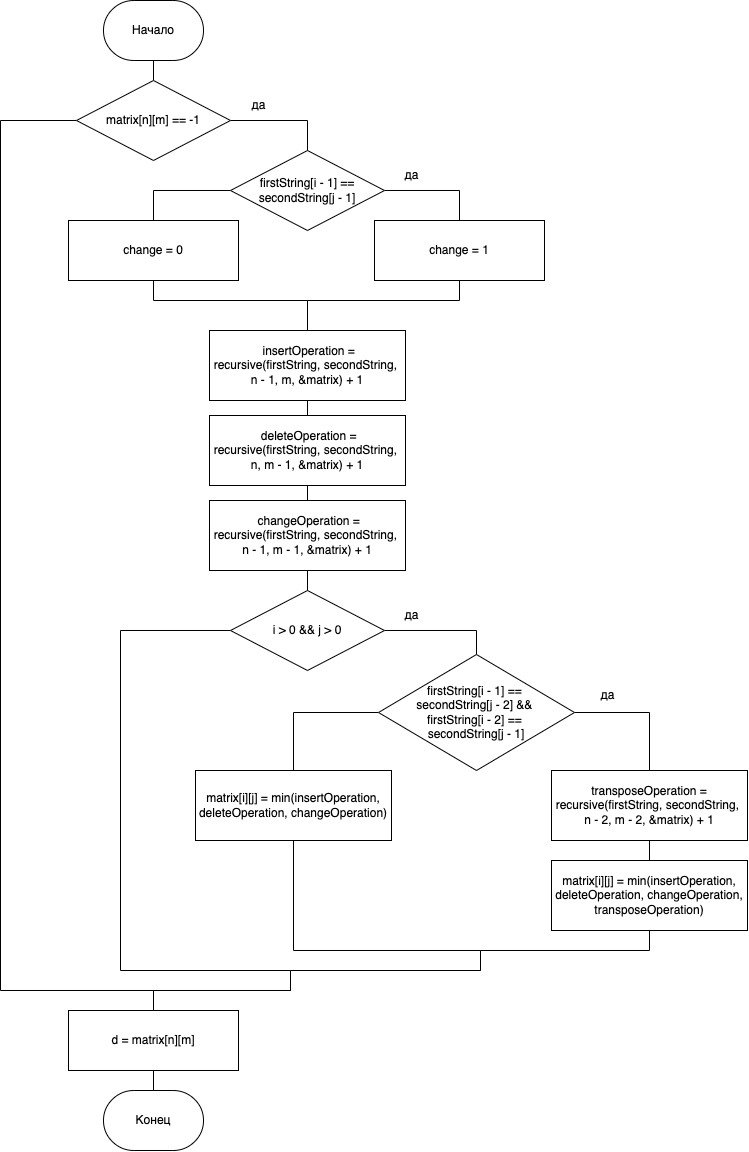
\includegraphics[scale=0.6]{img/dl_cash.png}
	\caption{Схема алгоритма Винограда}
	\label{fig:mpr}
\end{figure}

\pagebreak

\begin{figure}[ht!]
	\centering
	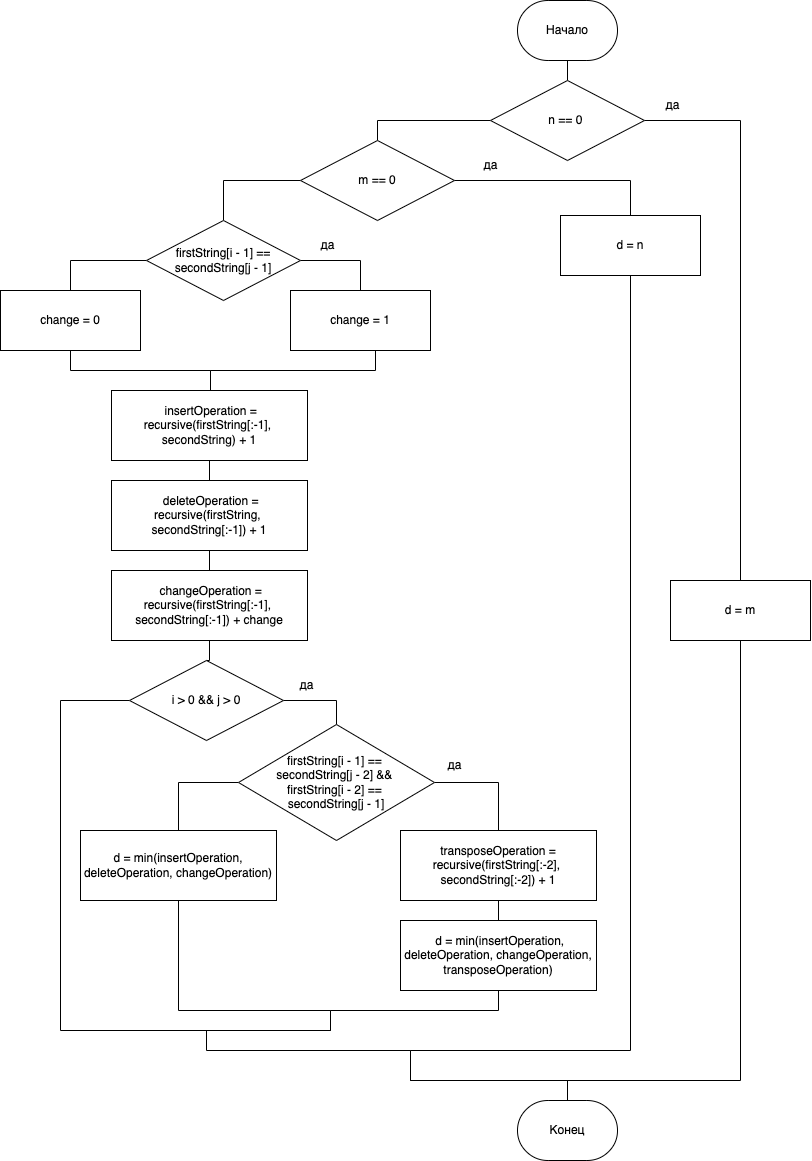
\includegraphics[scale=0.55]{img/dl_recursive.png}
	\caption{Схема функций оптимизированного алгоритма Винограда}
	\label{fig:mpr}
\end{figure}

\clearpage
